\section{Off-Chain Protocol}

We sate the coordinated off-chain protocol in Figure~\ref{fig:head_coordinated}.
Note the following deviations of the original protocol in~\cite{hydrahead20}.

\begin{itemize}
\item No hanging transactions due to `coordination'.
\item No acknowledgement nor confirmation of transactions.
\item No confirmation of snapshots (two-round confirmation by local acknowledgement).
\end{itemize}

Variables:

\begin{center}
\begin{tabular}{|l|l|}\hline
  $\hats$  & Sequence number of latest (possibly unconfirmed) snapshot. \\ \hline
  $\bars$  & Sequence number of latest confirmed snapshot. \\ \hline
  $\hatmU$ & Latest (possibly unconfirmed) snapshot object. \\ \hline
  $\barmU$ & Latest confirmed snapshot object. \\ \hline
  $\hatmL$ & Local ledger extension by next leader. Only the next leader
  makes use of this variable.\\ \hline
  $\mT$    & Set of all received transactions (independent of their validity).\\  \hline
  $\hatmT$ & Transactions that extend the next leader's $\barmU$ (or $\hatmU$) to form $\hatmL$.\\
           & Only the next leader makes use of this variable.\\  \hline
  $\barmT$ & Set of all confirmed transactions up to the latest confirmed snapshot.\\  \hline
\end{tabular}
\end{center}

In particular, note, that the original variables $\hatmT$ and $\barmT$ are not required anymore because they
were used in context of hanging transactions. We thus reused them to fit the new context.

\begin{figure*}[t!]

  \def\sfact{0.8}
  \centering
  \begin{algobox}{Coordinated Hydra Head}
    \medskip
    \begin{tabular}{c}
      %%% Initializing the head
      \begin{tabular}{cc}
        \adjustbox{valign=t,scale=\sfact}{
         \begin{walgo}{0.6}
          %%% INIT
           \On{$(\hpInit,\hydraKeys,\hydraSigningKey,\cardanoKeys,\cPer)$ from client}{ %
             $\hydraKeysAgg^{setup} \gets \msCombVK(\hydraKeys)$ \; %
             $\cardanoKeys^{setup} \gets \cardanoKeys$ \; %
             $\cPer^{setup} \gets \cPer$ \; %
            $\PostTx{}~(\mtxInit, \nop, \hydraKeysAgg,\cardanoKeys,\cPer)$ \; %
          }
          \vspace{12pt}

          \On{$(\gcChainInitial, \cid, \nop, \hydraKeysAgg, \cardanoKeys^{\#}, \cPer)$ from chain}{ %
           \Req{} $\hydraKeysAgg=\hydraKeysAgg^{setup}$\; %
           \Req{} $\cardanoKeys^{\#}= [ \hash(k)~|~\forall k \in \cardanoKeys^{setup}]$\; %
           \Req{} $\cPer=\cPer^{setup}$\; %
           % TODO: cid check good enough?
           \Req{} $\cid = \hash(\muHead(i_{seed}))$ \; %
          }
        \end{walgo}
        }
        &

        \adjustbox{valign=t,scale=\sfact}{
        \begin{walgo}{0.6}
          \On{$(\gcChainCommit, j, U)$ from chain}{ %
            $U_j \gets U $

            \If{$\forall k \in [1..n]: U_k \neq \undefined$}{ %
              $\eta \gets (0, \combine([U_1 \dots U_n]))$ \; %
              $\PostTx{}~(\mtxCCom, \eta)$ \; %
            } %
          }

          \vspace{12pt}

          \On{$(\gcChainCollectCom, \eta_{0})$ from chain}{ %
            \Req{} $\forall j \in [1..n]: U_j \neq \undefined$ \; %
            $\Uinit \gets \bigcup_{j=1}^{n} U_j$ \; %
            $\hatmU, \barmU, \hatmL \gets \Uinit$ \; %
            $\hats,\bars \gets 0$ \; %
            $\mT, \hatmT, \barmT \gets \emptyset$ \;
          }

        \end{walgo}
      }
      \end{tabular}
      
      \\
      \multicolumn{1}{l}{\line(1,0){490}} %
      \\

      %%% Open head
      \begin{tabular}{c@{}c}
        \adjustbox{valign=t,scale=\sfact}{
        \begin{walgo}{0.65}

          %%% NEW TX
          \On{$(\hpNew,\tx)$ from client}{%
            \Req{} $\validTx(\tx) \land \hatmL \applytx \tx \neq \bot$\;
            \Multi{} $(\hpRT,\tx)$%
          }

          \vspace{12pt}

          %%% REQ TX
          \On{$(\hpRT,\tx)$ from $\party_j$}{%
            \Req{} $\validTx(\tx) \land \hatmL \applytx \tx \neq \bot$ \;

            $\tx^{\#} \gets \hash(\tx)$ %

            $\mT \gets \mT \cup (\tx^{\#}, \tx)$ % all seen txs

            $\hatmT \gets \hatmT \cup (\tx^{\#}, \tx)$ % candidates for next snapshot

            $\hatmL \gets \hatmL\applytx\tx$ %

            % issue snapshot if we are leader
            \If{$\hats = \bars \land \hpLdr(\bars + 1) = i$}{%
              \Multi{} $(\hpRS,\bars+1,\hatmT^{\downarrow1})$ \;%
            }
          }

          \vspace{12pt} %

          %%% REQ SN
          %TODO: avoid hash resolution complexity? it's handwavy at best right now
          \On{$(\hpRS,s,\mT^{\#}_{req})$ from $\party_j$}{ %

            \Req{} $s = \hats + 1 \land \hpLdr(s) = j$ \; %


            % Wait for snapshot no snapshot in flight anymore and all txs resolvable
            \Wait{$\bars = \hats \land \forall h \in \mT^{\#}_{req} : (h, \cdot) \in \mT$}{ %

              % resolve requested transactions
              $\mT_{res} \gets [ \mT[h] ~ | ~ \forall h \in \mT^{\#}_{req}]$

              \Wait{$\barmU \applytx \mT_{res} \not= \bot$}{ %
                $\hats \gets \bars + 1$ \; %

                $\hatmU \gets \barmU \applytx \mT_{res}$ \; %

                $\eta' \gets (\hats, \combine(\hatmU))$ \; %
                $\msSig_i \gets \msSign(\hydraSigningKey, (\cid || \eta_{0} || \eta'))$ \; %
                $\hatSigma \gets \emptyset$

                $\Multi{}~(\hpAS,\hats,\msSig_i)$ \; %

                $\forall \tx \in \mT_{res}: \Out~(\hpSeen,\tx)$ \; %

                % TODO: pruning is handwavy
                $\hatmT :\subseteq_{\mbox{max}} \mT$ s.t. $\hatmU\applytx\hatmT\not=\bot$ \; %
                $\hatmL \gets \hatmU\applytx\hatmT$
              }
            }
           }
          
        \end{walgo}
        }
        &

        \adjustbox{valign=t,scale=\sfact}{
        \begin{walgo}{0.6}
          %%% ACK SN
          \On{$(\hpAS,s,\msSig_j)$ from $\party_j$}{ %

            \Req{} $s \in \{\hats,\hats+1\} ~ \land ~ (j,\msSig_j) \notin \hatSigma$
            \; %

            \Wait{$\hats=s$
            }{ %
            

            $\hatSigma \gets \hatSigma \cup (j,\msSig_j)$ \; %

            \If{$\forall k \in [1..n]: (k,\cdot) \in \hatSigma$}{ %
              $\msCSig \gets \msComb(\hydraKeys, \hatSigma)$ \; %

              $\eta' \gets (\hats, \combine(\hatmU))$ \; %
              \Req{} $\msVfy(\msCVK, (\cid || \eta_{0} || \eta'), \msCSig)$ \;
              $\barmU \gets \hatmU$ \; %
              $\bars \gets \hats$ \; %
              $\barsigma \gets \msCSig$ \; %

              $\forall \tx \in \mT_{res} : \Out (\hpConf,\tx)$ \; %

              % issue snapshot if we are leader
              \If{$\hats = \bars \land \hpLdr(\bars + 1) = i$}{%
                \Multi{} $(\hpRS,\bars+1,\hatmT^{\downarrow1})$ \;%
              }
            }
          } }
        \end{walgo}

          }

      \end{tabular}

      \\
      \multicolumn{1}{l}{\line(1,0){490}} %
      \\

      %%% Closing the head
      \begin{tabular}{c c}
        \adjustbox{valign=t,scale=\sfact}{
        \begin{walgo}{0.6}

          % CLOSE from client
          \On{$(\hpClose)$ from client}{ %
            $\eta' \gets (\bars, \combine(\barmU))$ \; %
            $\xi \gets \barsigma$ \; %
            $\PostTx{}~(\mtxClose, \eta', \xi)$ \; %
          }

        \end{walgo}
        }
        & \adjustbox{valign=t,scale=\sfact}{
          \begin{walgo}{0.6}

          \On{$(\gcChainClose, \eta) \lor (\gcChainContest, \eta)$ from chain}{ %
            $(s_{c}, \cdot) \gets \eta$ \;
            \If{$\bars > s_{c}$}{%
              $\eta' \gets (\bars, \combine(\barmU))$ \; %
              $\xi \gets \barsigma$ \; %
              $\PostTx{}~(\mtxContest, \eta', \xi)$ \; %
            } }

          \end{walgo}
          }
      \end{tabular}
    \end{tabular}
    \bigskip
  \end{algobox}
  
  \caption{Head-protocol machine for the \emph{coordinated head} from the
    perspective of party $\party_i$.}\label{fig:head_coordinated}

\end{figure*}



%%% Local Variables:
%%% mode: latex
%%% TeX-master: "main"
%%% End:


Comments: 
\begin{itemize}
\item Fix: from client or from network: same function called twice should trigger at most one wait.
  For instance, $\hpRS$ called twice must not queue the 'wait' part for multiple execution.
\item Fix: $\hpNS$ called twice must not trigger local $\hpRS$ twice.
\item Fix: Concurrency resolution (reqSn stack) for snapshots (see state diagram in \cite{hydraspec22}).
\item Add: garbage collection ($\hatmT,\barmT$,etc.)
\item Extensive code explanation (per line of code)
\end{itemize}

The following figure visualizes the possible event flows from the view of a single party.
\begin{figure}[ht]
  \centering
  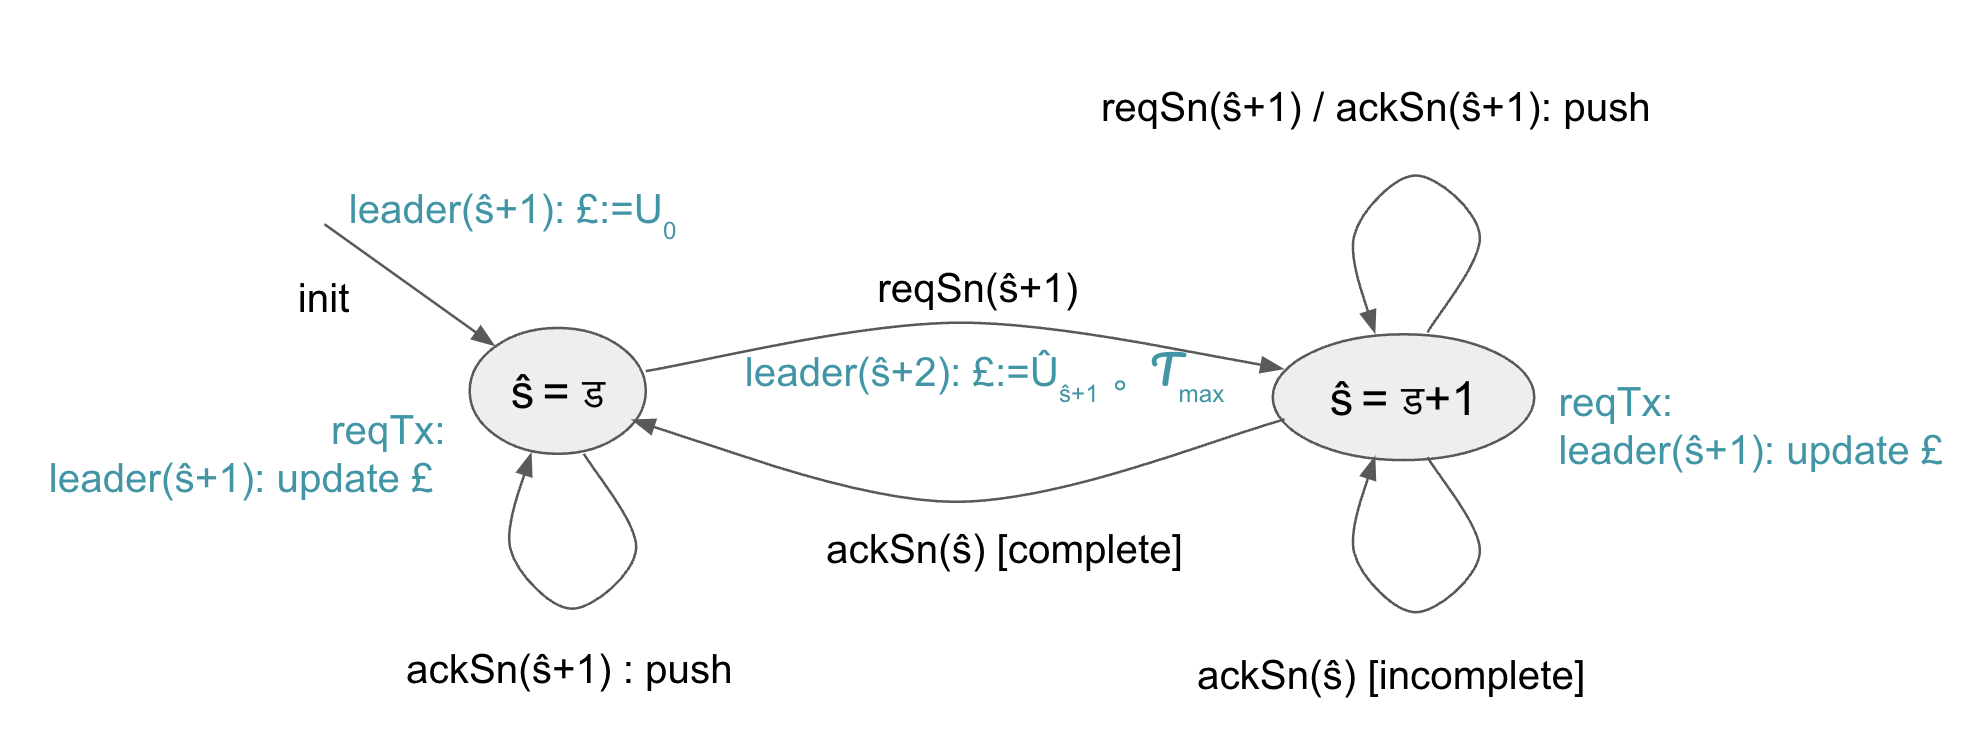
\includegraphics[width=\linewidth*2/3]{fig/reqackstates.png}
                  \caption{State diagram of reqSn/ackSn cycles.}
                  \label{fig:sim:baselines}
\end{figure}


